% !TEX encoding = UTF-8 Unicode
% !TEX root = ../report.tex
% 

\section{Construcción de la ontología}

\begin{figure}[h!]
  \makebox[\textwidth][c]{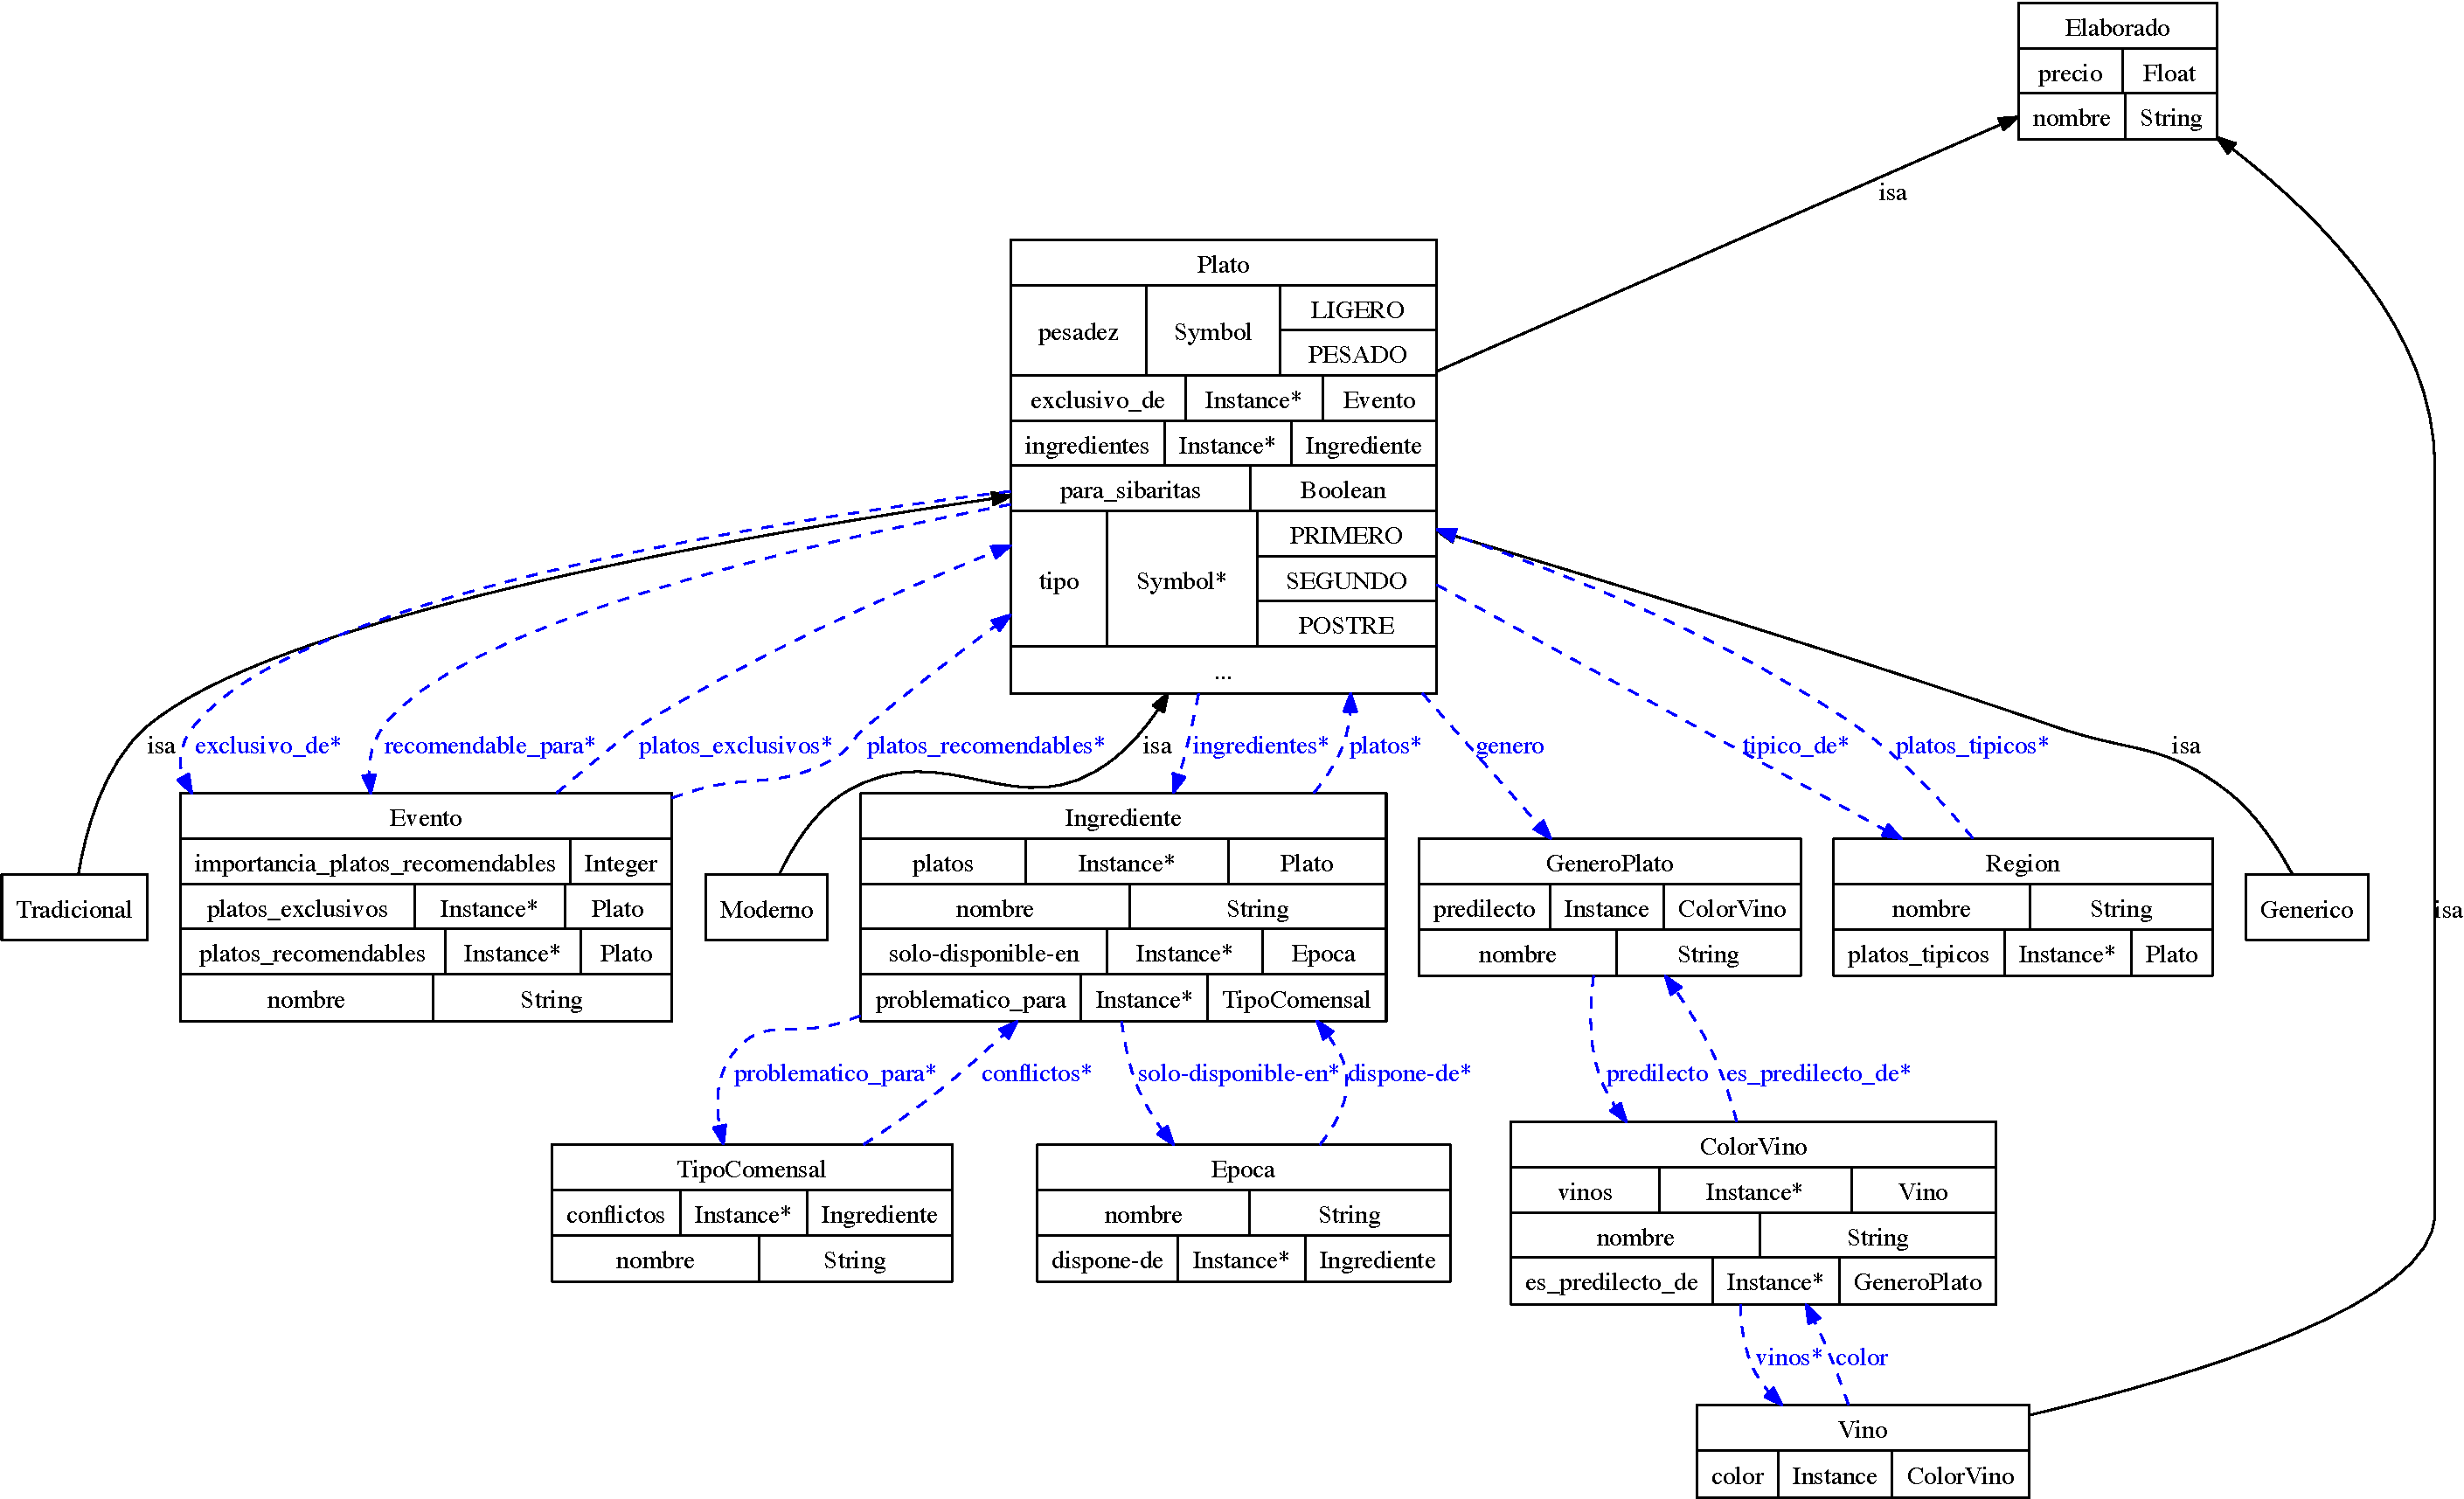
\includegraphics[width=1.2\textwidth]{%
      figures/ontologia}}
  \caption{La ontología final}
\end{figure}

La construcción de la ontología (y de todo el sistema en general) se ha
realizado de manera iterativa, aunque inicialmente no había sido así.

En un principio habíamos construido sistema de clases completo pero incluso más
complejo de lo que ha sido finalmente, sin necesidad. Afortunadamente, esa
versión se perdió y empezamos con una más simple que solamente contenía las
clases elaborado, plato, bebida (que ahora es solamente vino) e ingrediente.

Luego añadimos la clase de tipos de comensal, para poder tener en cuenta
alergias y demás problemas alimenticios. También se añadió la clase época para
poder indicar la disponibilidad de ingredientes.

Inicialmente, los eventos iban a ser unos valores prefijados hasta que vimos
que podríamos sacarle más provecho a todo si eran instancias dentro de la
ontología. Así que creamos la clase evento y asociamos algunos platos como
preferidos en el evento. Para evitar que determinados platos propios de un
evento se recomendaran en otros donde no tuviera sentido (un claro ejemplo son
los pasteles de boda), casi al final hicimos la diferencia entre platos propios
y platos que son recomendables para los eventos.

Ya, más entrados en el proceso de implementación del sistema experto, añadimos
la clase región para poder modelar el origen geográfico/cultural de los
platos. Finalmente, cuando empezamos a tratar con los vinos, y tras considerar
que la bebida en general no tiene sentido para el problema que se nos pide
resolver, eliminamos la clase bebida, dejando solamente una clase para
vinos. Además, creamos la clase que modela el color del vino, que se asoció a
la nueva clase de géneros de plato (sopa, pescado, estofado, aperitivo, etc.)
para poder hacer la recomendación de vinos de manera más sencilla.

Fuera de aquí, también están las ontologías de solución del problema, que
solamente contienen las clases menú y menú abstracto. Más adelante detallaremos
su funcionamiento.

\subsection{Detalle de las clases de la ontología del problema}
\subsubsection{Clase \texttt{Elaborado}}
Esta clase está construida para agrupar las características propias de los
productos que se venden con el menú: el \strong{nombre} y el
\strong{precio}. La idea es que cualquier cosa que esté en el menú debe ser un
producto elaborado.

En determinado momento tuvimos que hacer esta clase concreta para poder hacer
\emph{pattern matching} con CLIPS. Por suerte, los cambios que fuimos haciendo
en la implementación del problema provocaron que esta clase pudiera volver a
ser abstracta. Mientras la clase fue concreta, la clase \verb+Plato+ también
tuvo que serlo porque CLIPS no permite subclases abstractas de clases
concretas.

\subsubsection{Clase \texttt{Plato} y sus subclases}
La clase es abstracta y está dividida en las subclases \verb+Generico+,
\verb+Moderno+ y \verb+Tradicional+. Hemos decidido hacer esta clasificación
porque no es habitual que un plato sea moderno y tradicional a la vez, y
también existen platos que no se considerarían tradicionales pero que son
platos que se consumen habitualmente (de ahí el término genérico).

Además del nombre y el precio derivados de \verb+Elaborado+, la clase
\verb+Plato+ proporciona nuevos campos:
\begin{description}
\item[ingredientes] Es un campo múltiple de instancias de la clase
  \verb+Ingrediente+. Es necesario que haya como mínimo un ingrediente.
\item[genero] Es un campo simple que apunta a una instancia de
  \verb+GeneroPlato+. Sirve para clasificar los platos en sus géneros.
\item[tipo] Un campo múltiple que indica si el plato es \emph{primero},
  \emph{segundo} o \emph{postre}. Es necesario que sea algún tipo de plato.
\item[para\_sibaritas] Un campo cierto/falso. Los platos para sibaritas no
  queremos que se recomienden a alguien que no lo es, pues es habitual que no
  lo quieran. Por otro lado, se les da prioridad si el cliente sí lo es.
\item[temperatura] Indica si el plato es frío o caliente.
\end{description}
